\documentclass[11pt]{article}

%% MinionPro fonts 
%\usepackage[lf]{MinionPro}
%\usepackage{MnSymbol}
\usepackage{microtype}

%% Margins
\usepackage{geometry}
\geometry{verbose,letterpaper,tmargin=1in,bmargin=1in,lmargin=1in,rmargin=1in}

%% Other packages
\usepackage{amsmath}
\usepackage{amsthm}
\usepackage{amsfonts}
\usepackage[shortlabels]{enumitem}
\usepackage{titlesec}
\usepackage{soul}
\usepackage{tikz}
\usepackage{mathtools}
\usepackage{pgfplots}
\usepackage{tikz-3dplot}
\usepackage{algorithmic}
\usepackage[export]{adjustbox}
\usepackage{tcolorbox}
\usepackage{xcolor}
\usepackage{optprog}
\newcommand{\blu}{\color{blue}}
%% Paragraph style settings
\setlength{\parskip}{\medskipamount}
\setlength{\parindent}{0pt}

%% Change itemize bullets
\renewcommand{\labelitemi}{$\bullet$}
\renewcommand{\labelitemii}{$\circ$}
\renewcommand{\labelitemiii}{$\diamond$}
\renewcommand{\labelitemiv}{$\cdot$}

%% Colors
\definecolor{rred}{RGB}{204,0,0}
\definecolor{ggreen}{RGB}{0,145,0}
\definecolor{yyellow}{RGB}{255,185,0}
\definecolor{bblue}{rgb}{0.2,0.2,0.7}
\definecolor{ggray}{RGB}{190,190,190}
\definecolor{ppurple}{RGB}{160,32,240}
\definecolor{oorange}{RGB}{255,165,0}

%% Shrink section fonts
\titleformat*{\section}{\normalsize\bf}
\titleformat*{\subsection}{\normalsize\bf}
\titleformat*{\subsubsection}{\normalsize\it}

% %% Compress the spacing around section titles
\titlespacing*{\section}{0pt}{1.5ex}{0.75ex}
\titlespacing*{\subsection}{0pt}{1ex}{0.5ex}
\titlespacing*{\subsubsection}{0pt}{1ex}{0.5ex}

%% amsthm settings
\theoremstyle{definition}
\newtheorem{problem}{Problem}
\newtheorem{example}{Example}
\newtheorem*{theorem}{Theorem}
\newtheorem*{bigthm}{Big Theorem}
\newtheorem*{biggerthm}{Bigger Theorem}
\newtheorem*{bigcor1}{Big Corollary 1}
\newtheorem*{bigcor2}{Big Corollary 2}

%% tikz settings
\usetikzlibrary{calc}
\usetikzlibrary{patterns}
\usetikzlibrary{decorations}
\usepgfplotslibrary{polar}

%% algorithmic setup
\algsetup{linenodelimiter=}
\renewcommand{\algorithmiccomment}[1]{\quad// #1}
\renewcommand{\algorithmicrequire}{\emph{Input:}}
\renewcommand{\algorithmicensure}{\emph{Output:}}

%% Answer box macros
%% \answerbox{alignment}{width}{height}
\newcommand{\answerbox}[3]{%
  \fbox{%
    \begin{minipage}[#1]{#2}
      \hfill\vspace{#3}
    \end{minipage}
  }
}

%% \answerboxfull{alignment}{height}
\newcommand{\answerboxfull}[2]{%
  \answerbox{#1}{6.38in}{#2} 
}

%% \answerboxone{alignment}{height} -- for first-level bullet
\newcommand{\answerboxone}[2]{%
  \answerbox{#1}{6.0in}{#2} 
}

%% \answerboxtwo{alignment}{height} -- for second-level bullet
\newcommand{\answerboxtwo}[2]{%
  \answerbox{#1}{5.8in}{#2}
}

%% special boxes
\newcommand{\wordbox}{\answerbox{c}{1.2in}{.5cm}}
\newcommand{\catbox}{\answerbox{c}{.5in}{.7cm}}
\newcommand{\letterbox}{\answerbox{c}{.7cm}{.5cm}}

%% Miscellaneous macros
\newcommand{\tstack}[1]{\begin{multlined}[t] #1 \end{multlined}}
\newcommand{\cstack}[1]{\begin{multlined}[c] #1 \end{multlined}}
\newcommand{\ccite}[1]{\only<presentation>{{\scriptsize\color{gray} #1}}\only<article>{{\small [#1]}}}
\newcommand{\grad}{\nabla}
\newcommand{\ra}{\ensuremath{\rightarrow}~}
\newcommand{\maximize}{\text{maximize}}
\newcommand{\minimize}{\text{minimize}}
\newcommand{\subjectto}{\text{subject to}}
\newcommand{\trans}{\mathsf{T}}
\newcommand{\bb}{\mathbf{b}}
\newcommand{\bx}{\mathbf{x}}
\newcommand{\bc}{\mathbf{c}}
\newcommand{\bd}{\mathbf{d}}

%% LP format
%    \begin{align*}
%      \maximize \quad & \mathbf{c}^{\trans} \mathbf{x}\\
%      \subjectto \quad & A \mathbf{x} = \mathbf{b}\\
%                       & \mathbf{x} \ge \mathbf{0}
%    \end{align*}


%% Redefine maketitle
\makeatletter
\renewcommand{\maketitle}{
  \noindent SA405 -- AMP \hfill Rader \S 3.1 \\

  \begin{center}\Large{\textbf{\@title}}\end{center}
}
\makeatother

%% ----- Begin document ----- %%
\begin{document}
  
\title{Project 1:  Guiness}

\maketitle

\textbf{Part 1: Solution}

You may use my solution for your python implementation for part 2. If your own model is already correct, you can use it instead or make the necessary corrections.

\section{Network Diagram}

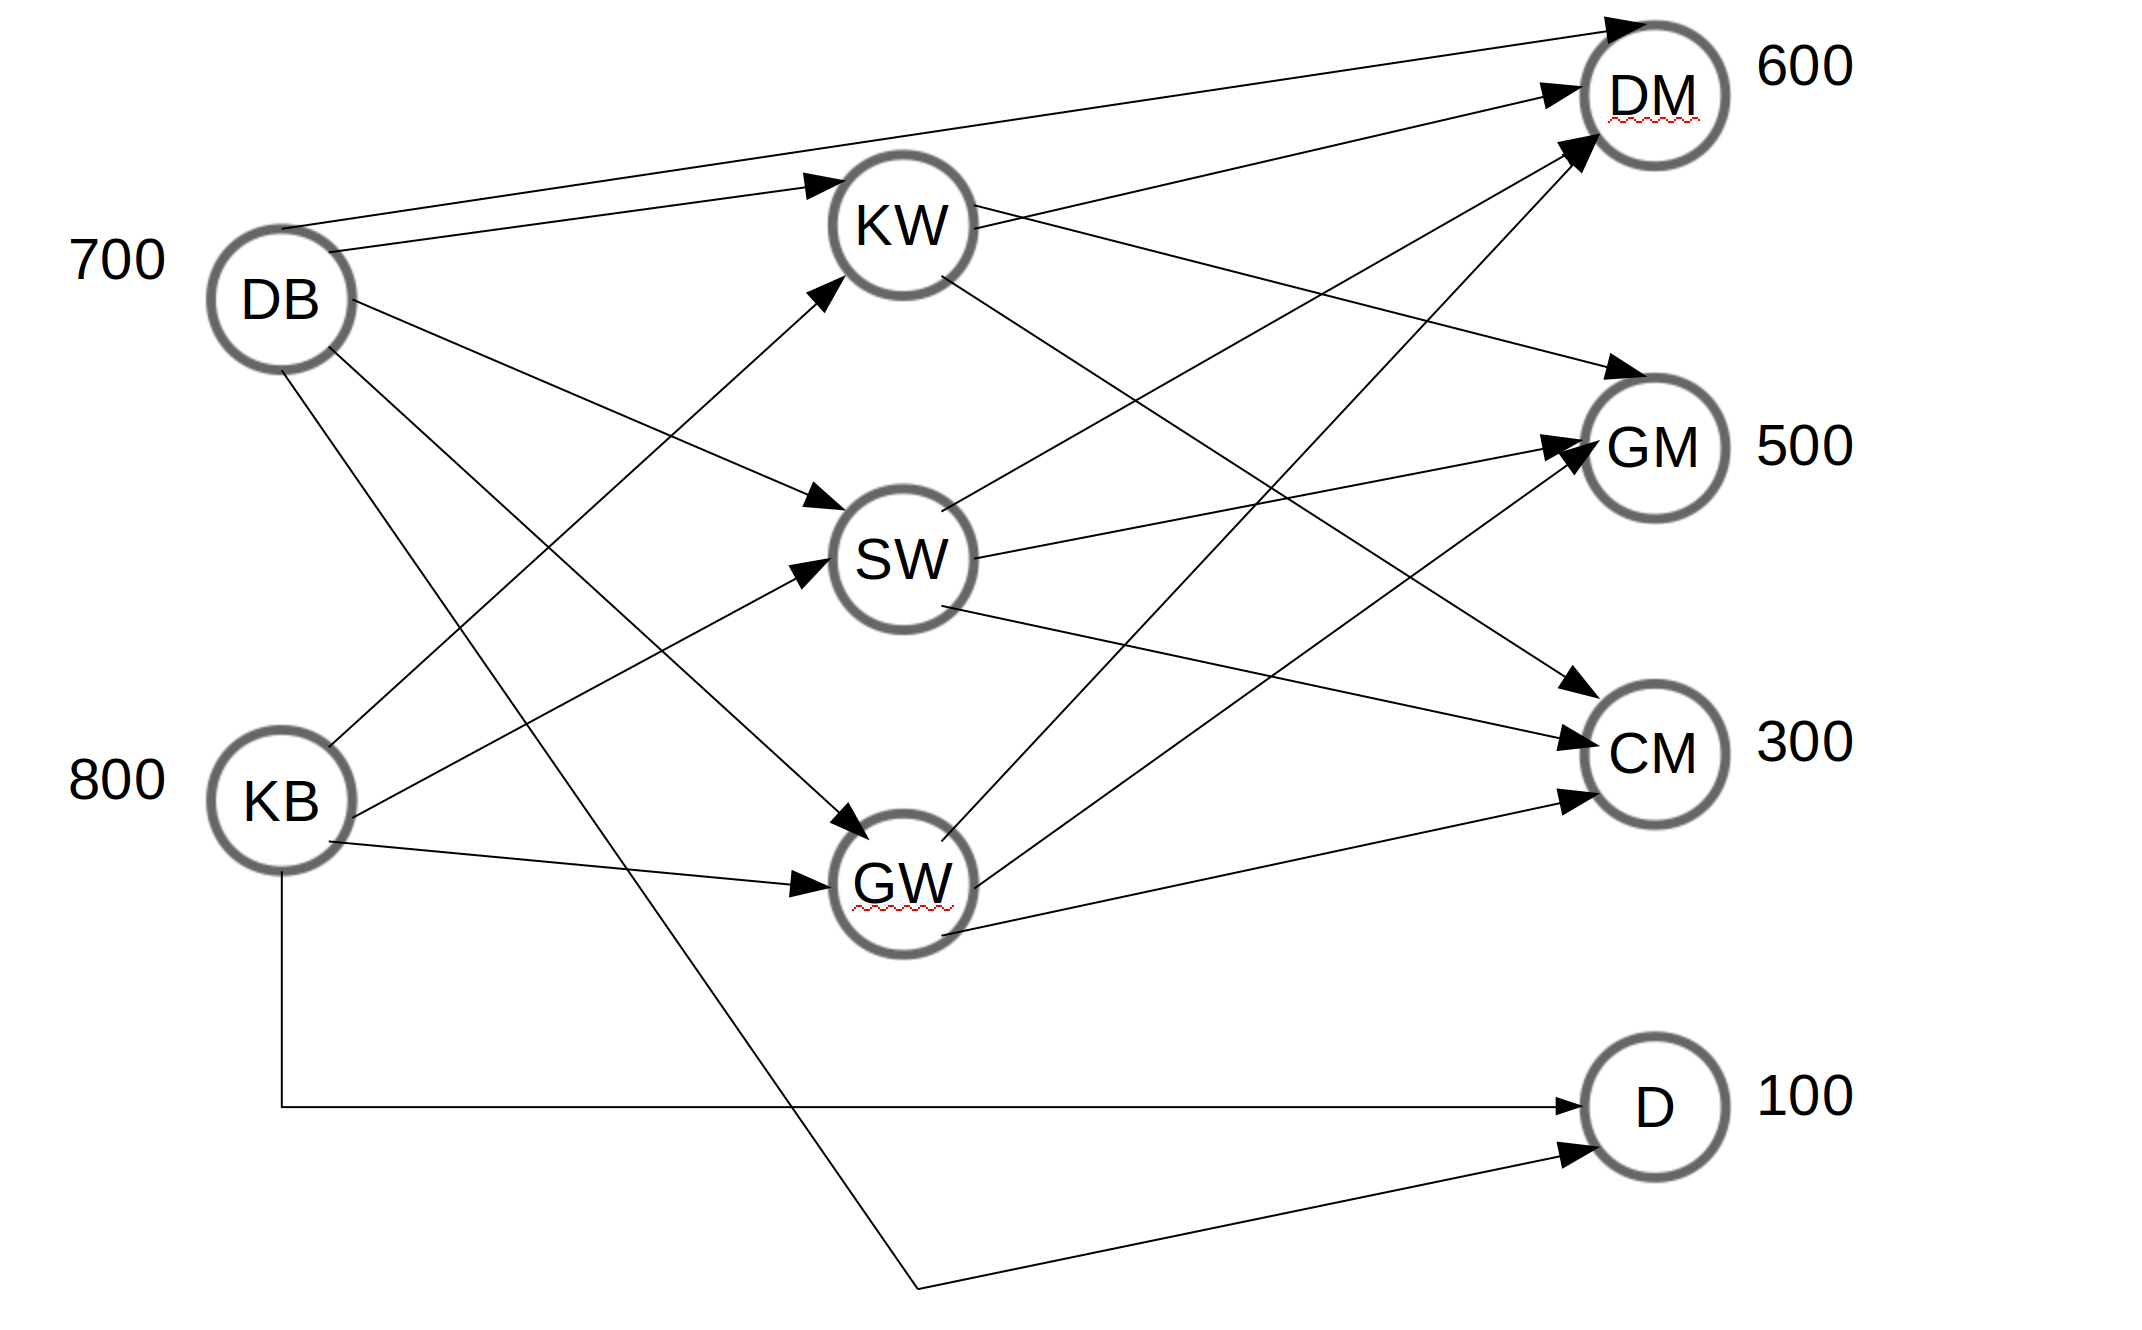
\includegraphics[width=0.9\textwidth]{Guiness-network.png}

\newpage

\section{Concrete Model}

\textbf{Decision Variables}

Let $x_{i,j}$ be the number of cases to transport from $i$ to $j$ for each edge $(i,j)$

Let $z_i = 1$ if we use warehouse $i$ or $0$ if we do not for each $i \in \{KW, SW, GW\}$

\textbf{Objective Function}

\[
\text{minimize cost: } 15 x_{DB,KW} + 10 x_{DB,SW} + \cdots + 12 x_{GW,CM} + 240 z_{KW} + 450 x_{SW} + 320 z_{GW}
\]

\textbf{Constraints}

\begin{optprog*}
st & x_{DB,KW} + x_{KB,KW} = x_{KW,DM} + x_{KW,GM} + x_{KW,CM} &&& \text{(Flow in = Flow out at Kilgore)} \\
   & x_{DB,SW} + x_{KB,SW} = x_{SW,DM} + x_{SW,GM} + x_{SW,CM} &&& \text{(Flow in = Flow out at Sligo)} \\
   & x_{DB,GW} + x_{KB,GW} = x_{GW,DM} + x_{GW,GM} + x_{GW,CM} &&& \text{(Flow in = Flow out at Galway)} \\
   & x_{DB,KW} + x_{DB,SW} + x_{DB,GW} + x_{DB,DM} + x_{DB,D} & = & 700 & \text{(Supply at Dublin-B)} \\
   & x_{KB,KW} + x_{KB,SW} + x_{KB,GW} + x_{KB,D}          & = & 800 & \text{(Supply at Kilarny)} \\
   & x_{DB,DM} + x_{KW,DM} + x_{SW,DM} + x_{GW,DM} & = & 600 & \text{(Demand at Dublin-M)} \\
   & x_{KW,GM} + x_{SW,GM} + x_{GW,GM}  & = & 500 & \text{(Demand at Galway)} \\
   & x_{KW,CM} + x_{SW,CM} + x_{GW,CM}  & = & 300 & \text{(Demand at Cork)} \\
   & x_{DB,D} + x_{KB,D} & = & 100 & \text{(Demand at Dummy)} \\
   & x_{KW,DM} + x_{KW,GM} + x_{KW,CM} & \leq & 400 z_{KW} & \text{(Weak forcing constraint on Kilgore W)} \\
	& x_{SW,DM} + x_{SW,GM} + x_{SW,CM} & \leq & 800 z_{SW} & \text{(Weak forcing constraint on Sligo W)} \\   
	& x_{GW,DM} + x_{GW,GM} + x_{GW,CM} & \leq & 600 z_{GW} & \text{(Weak forcing constraint on Galway W)} \\
   & x_{DB,KW}, x_{DB,SW}, \cdots, x_{GW,CM} & \in & \mathbb{Z}^+ & \text{(Integrality)} \\
   & z_{KW}, z_{SW}, z_{GW} & \in & \{0,1\} & \text{(Binary)}
\end{optprog*}

\newpage

\section{Parameterized Model}


\textbf{Sets}

Let $E$ be the set of edges \\
Let $W$ be the set of warehouses \\
Let $N$ be the set of nodes

\textbf{Decision Variables}

Let $x_{i,j}$ be the units shipped along edge $(i,j) \in E$ \\
Let $z_w = 1$ if warehouse $w$ is open and 0 otherwise for all $w \in W$

\textbf{Parameters} 

Let $c_{i,j}$ be the cost of sending one unit along edge $(i,j)$ for all $(i,j) \in E$. \\
Let $f_w$ be the fixed cost of opening warehouse $w$ for all $w \in W$ \\
Let $s_i$ be the supply of node $i$ for all $i \in N$ \\
Let $d_i$ be the demand of node $i$ for all $i \in N$ \\
Let $M_w$ be the capacity of warehouse $w$ for all $w \in W$ \\

\textbf{Objective Function}

\[
\text{minimize cost: } \sum_{(i,j) \in E} c_{i,j} x_{i,j}  + \sum_{w \in W} f_w z_w
\]

\textbf{Constraints}

\begin{optprog*}
st & \sum_{ (i,n) \in E} x_{i,n} + s_n & = & \sum_{(n,j) \in E} x_{n,j} + d_n & \text{for $n \in N$} & \text{(Flow balance of each node)} \\
   & \sum_{(i,w) \in E} x_{i,w} & \leq & M_w z_w & \text{for all $w \in W$} & \text{(forcing and capacity constraints)} \\
   & x_{i,j} & \in & \mathbb{Z}^+ & \text{for all $(i,j) \in E$} & \text{(Integrality)} \\
   & z_w & \in & \{0,1\} & \text{for all $w \in W$} & \text{(Binary)}
\end{optprog*}

\textbf{Note:} You can replace the weak forcing constraints with strong forcing constraints. But if you do this, you still have to account for the capacities by putting a bound on the flow in or flow out of each warehouse.

\end{document}
